longitud
\section{Análisis de resultados}

Tras realizar las distintas pruebas y ejecuciones, utilizando tanto el algoritmo de Programación Genética como GA-P, así como el conjunto de datos original como el conjunto de datos sobremuestreado, en esta sección analizaremos los resultados obtenidos. En este análisis nos centraremos en los siguientes apartados:

\begin{enumerate}
	\item \textbf{Comparación del uso de distintas longitudes de árbol.} Estudiaremos si es necesario utilizar árboles con muchos nodos, de cara a que el algoritmo se pueda ajustar tanto como desee, o si por el contrario el ser menos restrictivos con la longitud conlleva a un sobreajuste por parte del modelo.
	\item \textbf{Comparación entre Programación Genética y GA-P.} Compararemos los resultados entre ambos algoritmos, viendo sus diferencias así como comentar si para este problema ha funcionado las adaptaciones que aplica GA-P al algoritmo original de Programación Genética.
	\item \textbf{Comparación entre los resultados obtenidos por el conjunto de datos original y el conjunto de datos con sobremuestreo.} En este caso veremos si es necesario aplicar las técnicas de sobremuestreo, si han mejorado los resultados de forma notable y por lo tanto se debería tener en cuenta para trabajos futuros con este conjunto de datos, donde la falta de balanceo de datos es clara.
	\item \textbf{Comparación de los resultados obtenidos con el estado del arte.} Finalmente revisaremos el estado del arte, compararemos nuestros resultados con los estudios previos, y comentaremos si este enfoque ha proporcionado un nuevo punto de vista viable para abordar el problema de estimación de la edad.
	\item \textbf{Estudio de las mejores expresiones obtenidas.} Se escogerán las mejores expresiones obtenidas de todas las ejecuciones, así como un estudio de estas, como obtener las características que Programación Genética y GA-P han tenido más en cuenta para obtener los resultados.
\end{enumerate}


\subsection{Resumen de los resultados}

Para realizar el análisis de resultados, debido a la gran cantidad de ejecuciones realizadas y resultados obtenidos, se han resumidos los resultados en seis tablas, una tabla por conjunto de datos (diferenciando entre conjunto original y con sobremuestreo), donde podemos ver los errores en media de cada algoritmo con distinta longitud máxima de árbol.


\begin{table}[H]
\centering
\resizebox{\textwidth}{!}{%
\begin{tabular}{|c|c|c|c|c|}
\hline
\multicolumn{5}{|c|}{\textbf{Comparación de las ejecuciones sobre la lateralidad izquierda}}                      \\ \hline
\textbf{}                            & \textbf{ECM con 5x2-cv} & \textbf{RECM con 5x2cv} & \textbf{MAE con 5x2cv} & \textbf{Tiempo de ejecución (s)}\\ \hline
\textbf{PG: Longitud máxima 20}   & 78,29122                & 8,840838                & 7,34858                & 211,616\\ \hline
\textbf{PG: Longitud máxima 40}   & 83,53466                & 8,97871                 & 7,283056               & 373,8546\\ \hline
\textbf{PG: Longitud máxima 60}   & 78,26134                & 8,82909                 & 7,26459                & 520,019\\ \hline
\textbf{GA-P: Longitud máxima 20} & 77,69454                & 8,807858                & 7,310698               & 283,5206\\ \hline
\textbf{GA-P: Longitud máxima 40} & 75,86876                & 8,704602                & 7,226134               & 499,1296\\ \hline
\textbf{GA-P: Longitud máxima 60} & 78,14404                & 8,826406                & 7,281462               & 688,3636\\ \hline
\end{tabular}%
}
\caption{Resumen de los resultados obtenidos de media en la lateralidad izquierda.}\label{table:resumen_l0}
\end{table}


\begin{table}[H]
\centering
\resizebox{\textwidth}{!}{%
\begin{tabular}{|c|c|c|c|c|}
\hline
\multicolumn{5}{|c|}{\textbf{Comparación de las ejecuciones sobre la lateralidad derecha}}                        \\ \hline
\textbf{}                            & \textbf{ECM con 5x2-cv} & \textbf{RECM con 5x2cv} & \textbf{MAE con 5x2cv} & \textbf{Tiempo de ejecución (s)}\\ \hline
\textbf{PG: Longitud máxima 20}   & 72,09066                & 8,483666                & 6,963514               & 213,0604\\ \hline
\textbf{PG: Longitud máxima 40}   & 71,68338                & 8,45994                 & 6,92191                & 391,2276\\ \hline
\textbf{PG: Longitud máxima 60}   & 75,84564                & 8,647456                & 6,975748               & 533,1198\\ \hline
\textbf{GA-P: Longitud máxima 20} & 71,10252                & 8,425564                & 6,93037                & 283,6592\\ \hline
\textbf{GA-P: Longitud máxima 40} & 71,65424                & 8,457206                & 6,920638               & 517,811\\ \hline
\textbf{GA-P: Longitud máxima 60} & 72,13152                & 8,486486                & 6,94396                & 706,0454\\ \hline
\end{tabular}%
}
\caption{Resumen de los resultados obtenidos de media en la lateralidad derecha.}\label{table:resumen_l1}
\end{table}



\begin{table}[H]
\centering
\resizebox{\textwidth}{!}{%
\begin{tabular}{|c|c|c|c|c|}
\hline
\multicolumn{5}{|c|}{\textbf{Comparación de las ejecuciones sobre el conjunto de datos completo}}                      \\ \hline
\textbf{}                            & \textbf{ECM con 5x2-cv} & \textbf{RECM con 5x2cv} & \textbf{MAE con 5x2cv} & \textbf{Tiempo de ejecución (s)}\\ \hline
\textbf{PG: Longitud máxima 20}   & 73,50034                & 8,569666                & 7,065968               & 349,5058\\ \hline
\textbf{PG: Longitud máxima 40}   & 72,58126                & 8,515504                & 7,020512               & 662,9214\\ \hline
\textbf{PG: Longitud máxima 60}   & 71,4802                 & 8,450386                & 6,94271                & 940,1766\\ \hline
\textbf{GA-P: Longitud máxima 20} & 74,05094                & 8,599972                & 7,122182               & 460,3008\\ \hline
\textbf{GA-P: Longitud máxima 40} & 72,47752                & 8,510716                & 7,022764               & 875,7186\\ \hline
\textbf{GA-P: Longitud máxima 60} & 72,23008                & 8,494072                & 6,99007                & 1222,924\\ \hline
\end{tabular}%
}
\caption{Resumen de los resultados obtenidos de media en el conjunto de datos completo.}\label{table:resumen_completo}
\end{table}





\begin{table}[H]
\centering
\resizebox{\textwidth}{!}{%
\begin{tabular}{|c|c|c|c|c|}
\hline
\multicolumn{5}{|c|}{\textbf{Comparación de las ejecuciones sobre la lateralidad izquierda con sobremuestreo}}    \\ \hline
\textbf{}                            & \textbf{ECM con 5x2-cv} & \textbf{RECM con 5x2cv} & \textbf{MAE con 5x2cv} & \textbf{Tiempo de ejecución (s)}\\ \hline
\textbf{PG: Longitud máxima 20}   & 63,87642                & 7,987276                & 6,504278               & 261,74\\ \hline
\textbf{PG: Longitud máxima 40}   & 63,64042                & 7,9709                  & 6,466798               & 476,78\\ \hline
\textbf{PG: Longitud máxima 60}   & 63,17712                & 7,94391                 & 6,477742               & 657,799\\ \hline
\textbf{GA-P: Longitud máxima 20} & 63,67778                & 7,97497                 & 6,508852               & 345,7916\\ \hline
\textbf{GA-P: Longitud máxima 40} & 62,47418                & 7,90087                 & 6,43548                & 635,3626\\ \hline
\textbf{GA-P: Longitud máxima 60} & 68,1283                 & 8,148552                & 6,51231                & 879,1732\\ \hline
\end{tabular}%
}
\caption{Resumen de los resultados obtenidos de media en la lateralidad izquierda con sobremuestreo.}\label{table:resumen_l0_over}
\end{table}



\begin{table}[H]
\centering
\resizebox{\textwidth}{!}{%
\begin{tabular}{|c|c|c|c|c|}
\hline
\multicolumn{5}{|c|}{\textbf{Comparación de las ejecuciones sobre la lateralidad derecha con sobremuestreo}}      \\ \hline
\textbf{}                            & \textbf{ECM con 5x2-cv} & \textbf{RECM con 5x2cv} & \textbf{MAE con 5x2cv} & \textbf{Tiempo de ejecución (s)}\\ \hline
\textbf{PG: Longitud máxima 20}   & 67,82148                & 8,22918                 & 6,768058               & 257,7232\\ \hline
\textbf{PG: Longitud máxima 40}   & 68,17448                & 8,250954                & 6,791658               & 477,6992\\ \hline
\textbf{PG: Longitud máxima 60}   & 68,19856                & 8,252648                & 6,77378                & 680,5406\\ \hline
\textbf{GA-P: Longitud máxima 20} & 68,3044                 & 8,259594                & 6,826746               & 342,6014\\ \hline
\textbf{GA-P: Longitud máxima 40} & 67,7971                 & 8,227468                & 6,78825                & 622,9388\\ \hline
\textbf{GA-P: Longitud máxima 60} & 67,57086                & 8,214506                & 6,769916               & 882,5354\\ \hline
\end{tabular}%
}
\caption{Resumen de los resultados obtenidos de media en la lateralidad derecha con sobremuestreo.}\label{table:resumen_l1_over}
\end{table}



\begin{table}[H]
\centering
\resizebox{\textwidth}{!}{%
\begin{tabular}{|c|c|c|c|c|}
\hline
\multicolumn{5}{|c|}{\textbf{Comparación de las ejecuciones sobre el conjunto de datos completo con sobremuestreo}}      \\ \hline
\textbf{}                            & \textbf{ECM con 5x2-cv} & \textbf{RECM con 5x2cv} & \textbf{MAE con 5x2cv} & \textbf{Tiempo de ejecución (s)}\\ \hline
\textbf{PG: Longitud máxima 20}   & 63,8009                 & 7,985344                & 6,55832                & 465,1212\\ \hline
\textbf{PG: Longitud máxima 40}   & 62,44686                & 7,899814                & 6,471976               & 898,2496\\ \hline
\textbf{PG: Longitud máxima 60}   & 62,2492                 & 7,887122                & 6,465792               & 1245,464\\ \hline
\textbf{GA-P: Longitud máxima 20} & 63,61904                & 7,97332                 & 6,553096               & 613,734\\ \hline
\textbf{GA-P: Longitud máxima 40} & 64,6985                 & 8,01656                 & 6,529756               & 1181,024\\ \hline
\textbf{GA-P: Longitud máxima 60} & 62,41038                & 7,897584                & 6,481414               & 1642,246\\ \hline
\end{tabular}%
}

\caption{Resumen de los resultados obtenidos de media en el conjunto de datos completo con sobremuestreo.}\label{table:resumen_completo_over}
\end{table}



\subsection{Uso de distintas longitudes en Programación Genética y GA-P}

Como podemos ver en cada ejecución de los distintos conjuntos en ambos algoritmos, las diferencias de resultados en un conjunto de datos con un algoritmo, variando únicamente la longitud máxima de los árboles a utilizar no son significantes.

En las tablas de la sección anterior (\ref{table:resumen_l0}, \ref{table:resumen_l1}, \ref{table:resumen_completo}, \ref{table:resumen_l0_over}, \ref{table:resumen_l1_over} y \ref{table:resumen_completo_over}) podemos ver como la longitud máxima de los nodos apenas influye en los resultados y las expresiones obtenidas por las ejecuciones con una longitud máxima de veinte nodos son mucho más sencillas de interpretar.

A pesar de esto, podemos encontrar algunas excepciones, como en la tabla \ref{table:resumen_completo_over}, donde vemos como tanto para Programación Genética como para GA-P utilizar el tamaño más grande si que se han conseguido mejores resultados. Con respecto a esto, en GA-P podemos ver que se trata de una excepción al ver que en los resultados en otras tablas siempre se obtiene el mejor valor con una longitud de veinte, y en los casos donde se obtiene el mejor valor con cuarenta nodos la diferencia es ínfima. Sin embargo para Programación Genética esto se repite en la mayoría de las tablas, como \ref{table:resumen_l0}, \ref{table:resumen_completo} o \ref{table:resumen_completo_over}. Comentaremos este detalle en la siguiente sección, donde comparamos Programación Genética y GA-P.

\newpage

\subsection{Comparación entre Programación Genética y GA-P}

Un primer detalle que podemos observar en los resultados, comentado en la sección anterior, es la diferencia entre Programación Genética y GA-P en los resultados comparando distintas longitudes máximas para los árboles. Programación Genética si que llega a obtener mejores resultados con una longitud de cuarenta nodos (aunque la diferencia sea muy pequeña), mientras que con GA-P si que llegamos a obtener buenos resultados con veinte nodos, lo que nos lleva a pensar que el ampliar la longitud máxima de las expresiones para Programación Genética si que ha beneficiado a los resultados. Esto se puede explicar fácilmente por la mejora que añade GA-P, ya que al ser capaz de aprender los valores constantes no necesita aplicar operaciones sobre dichas constantes para obtener ciertos valores, mientras que Programación Genética si, por lo que la mayor longitud máxima del árbol le permite ajustar más las constantes.

De cara a los resultados obtenidos, podemos ver como en la mayoría de las tablas GA-P obtiene mejores valores que Programación Genética, teniendo como única excepción la tabla \ref{table:resumen_completo_over}. De cara a observar estas distinciones también se han realizado las siguientes gráficas:

\begin{figure}[H]
    \centering
	  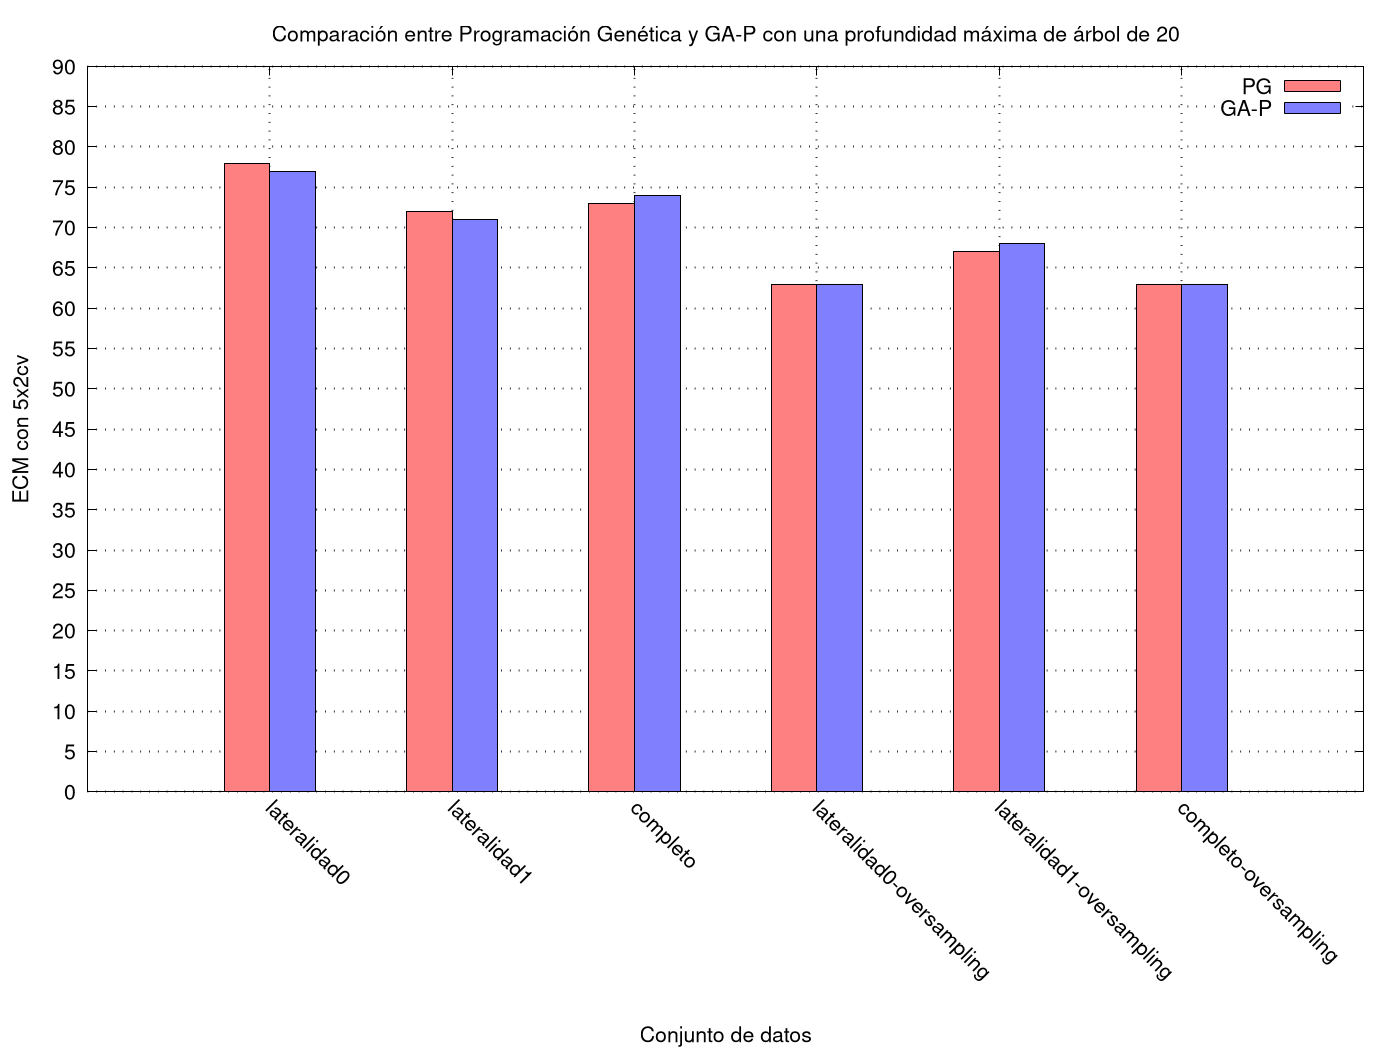
\includegraphics[width=0.7\textwidth]{analisis/comparacion_pg_gap_20.png}
	  \caption{Comparación entre PG y GA-P con longitud máxima de 20 nodos.}\label{fig:cmp_pg_gap_20}

\end{figure}

\begin{figure}[H]
    \centering
	  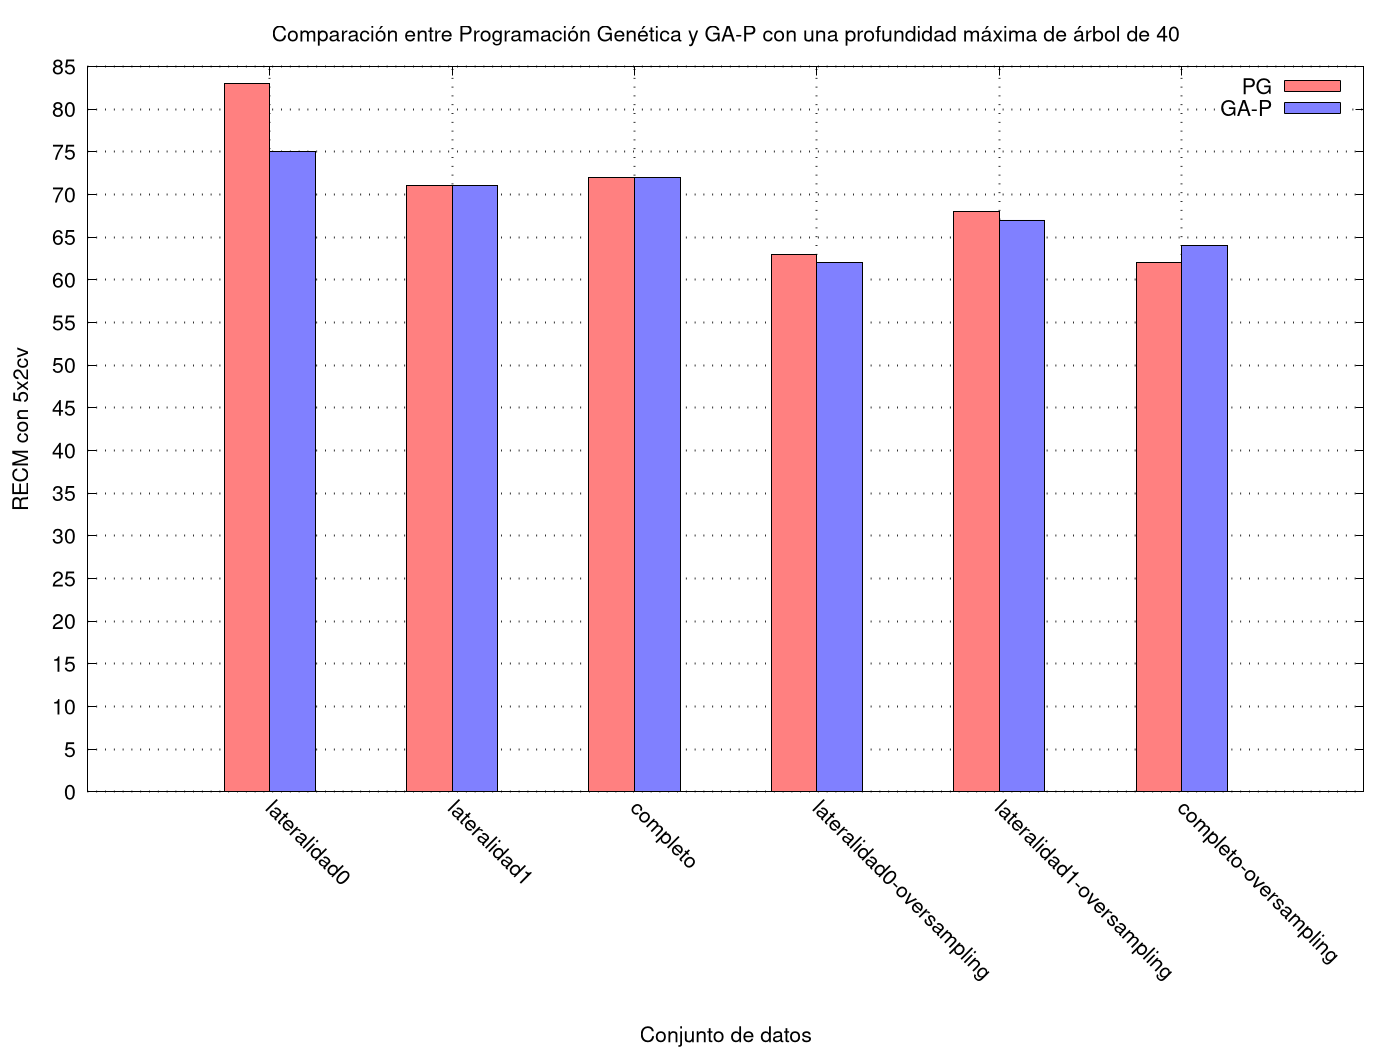
\includegraphics[width=0.7\textwidth]{analisis/comparacion_pg_gap_40.png}
	  \caption{Comparación entre PG y GA-P con longitud máxima de 40 nodos.}\label{fig:cmp_pg_gap_40}

\end{figure}

\begin{figure}[H]
    \centering
	  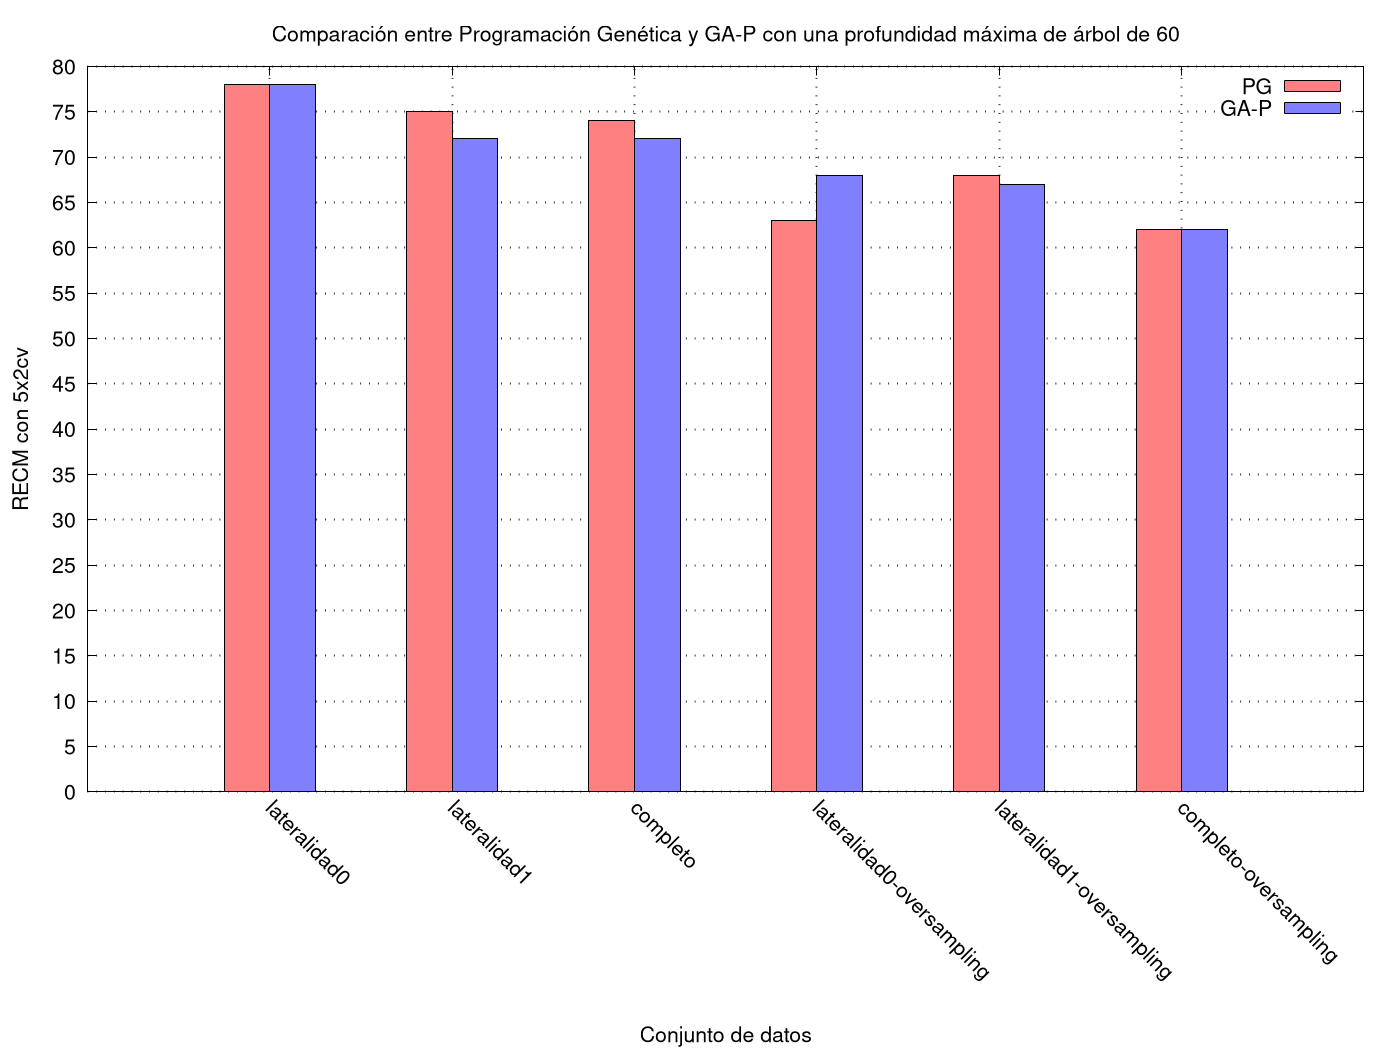
\includegraphics[width=0.7\textwidth]{analisis/comparacion_pg_gap_60.png}
	  \caption{Comparación entre PG y GA-P con longitud máxima de 60 nodos.}\label{fig:cmp_pg_gap_60}
\end{figure}



Las tablas \ref{table:resumen_l0}, \ref{table:resumen_l1} y \ref{table:resumen_completo} e imágenes \ref{fig:cmp_pg_gap_20}, \ref{fig:cmp_pg_gap_40} y \ref{fig:cmp_pg_gap_60} nos muestran como la mejora de GA-P se nota especialmente en los conjuntos de datos sin sobremuestreo, mientras que en los resultados con sobremuestreo esta diferencia es más pequeña, lo que nos lleva a pensar que GA-P es más versátil para conjuntos de datos donde existen pocas muestras para algunas etiquetas, adaptándose mejor que Programación Genética para problemas de regresión simbólica al implementar la mejora de nichos y aprender mejor la fórmula obtenida, ya que Programación Genética si que necesita más cantidad de datos para aprender la fórmula.

\subsection{Comparación de resultados del conjunto de datos original y del conjunto de datos con sobremuestreo}

Con respecto a los resultados obtenidos con el conjunto de datos original y el conjunto con datos sintéticos, podemos ver como claramente se consigue una mejora en los resultados:

\begin{figure}[H]
    \centering
	  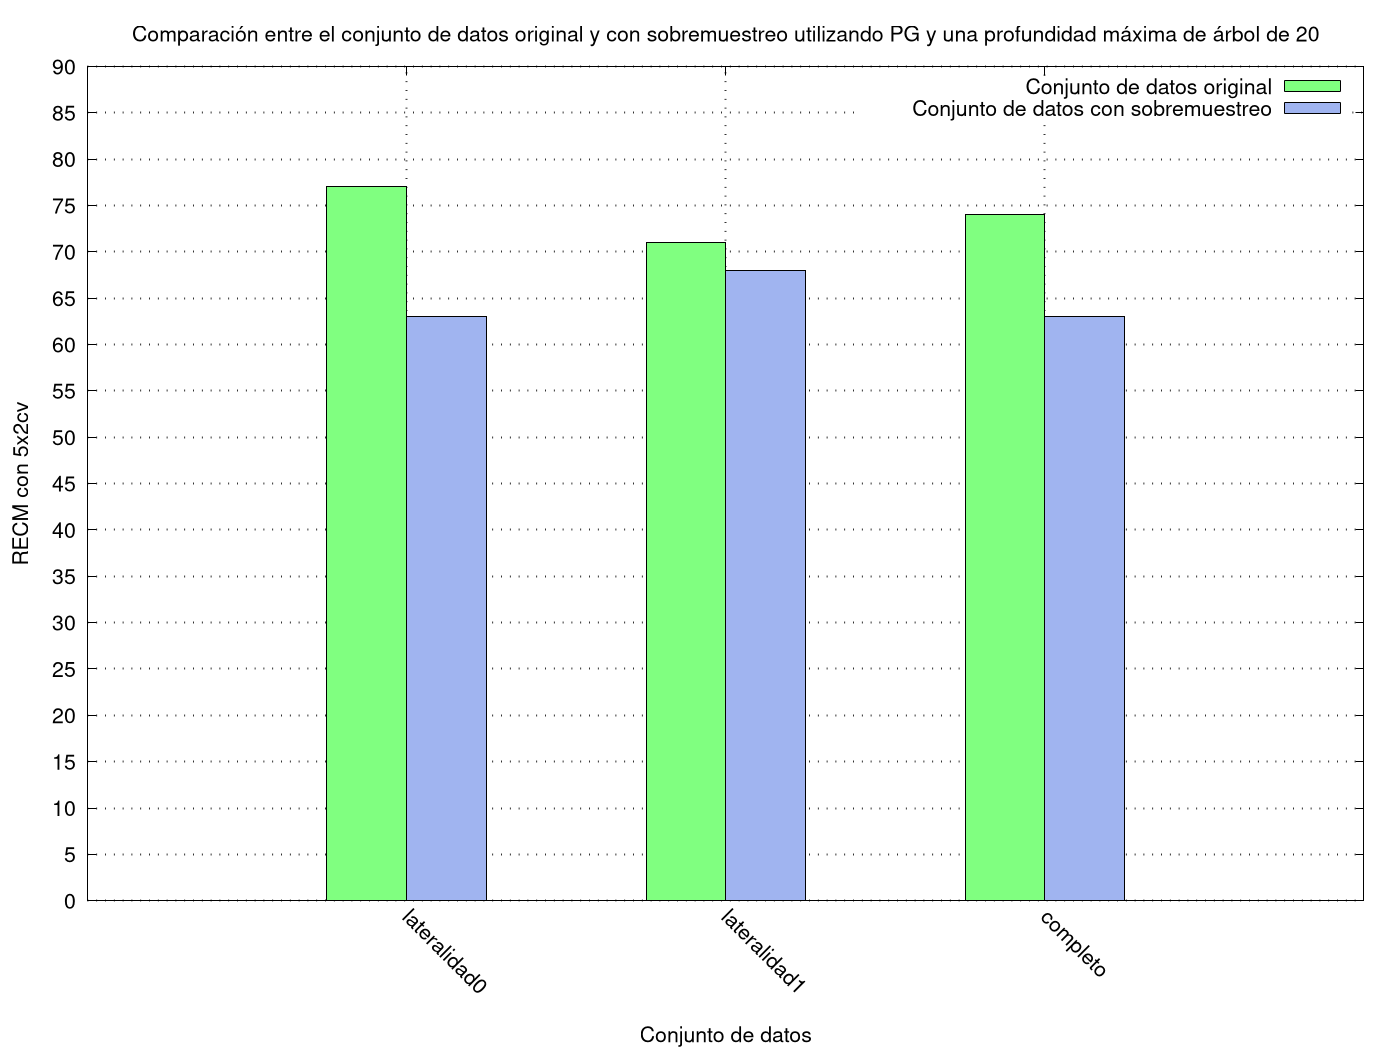
\includegraphics[width=0.7\textwidth]{analisis/comparacion_over_pg_20.png}
	  \caption{Comparación entre el conjunto de datos original y con sobremuestreo con PG y longitud máxima de 20 nodos.}\label{fig:cmp_pg_over_20}

\end{figure}

\begin{figure}[H]
    \centering
	  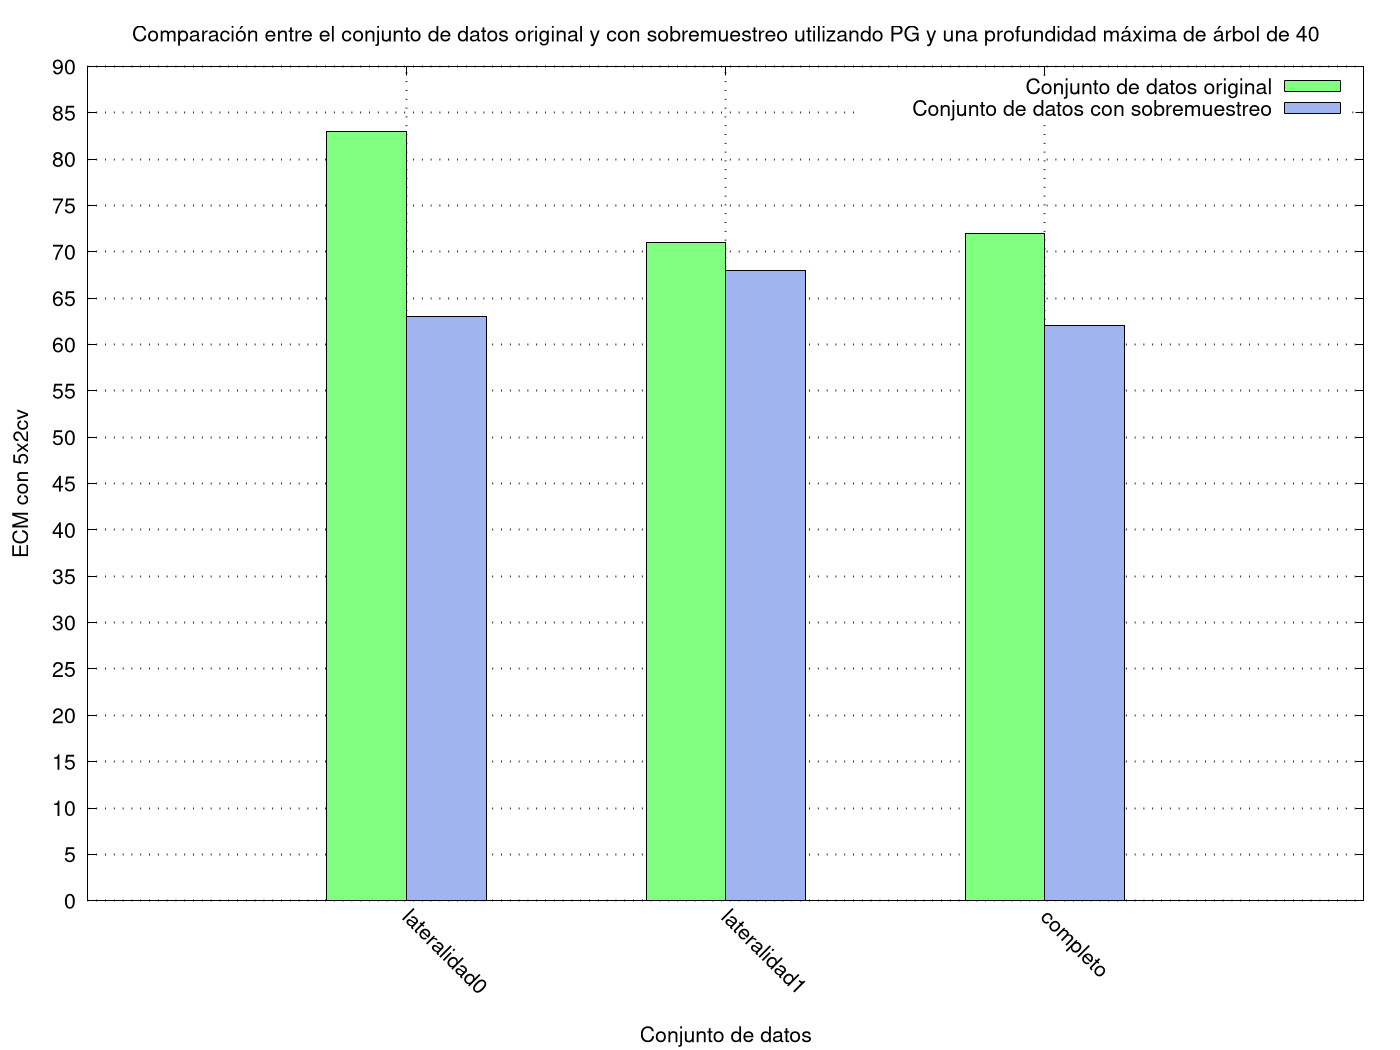
\includegraphics[width=0.7\textwidth]{analisis/comparacion_over_pg_40.png}
	  \caption{Comparación entre el conjunto de datos original y con sobremuestreo con PG y longitud máxima de 40 nodos.}\label{fig:cmp_pg_over_40}

\end{figure}

\begin{figure}[H]
    \centering
	  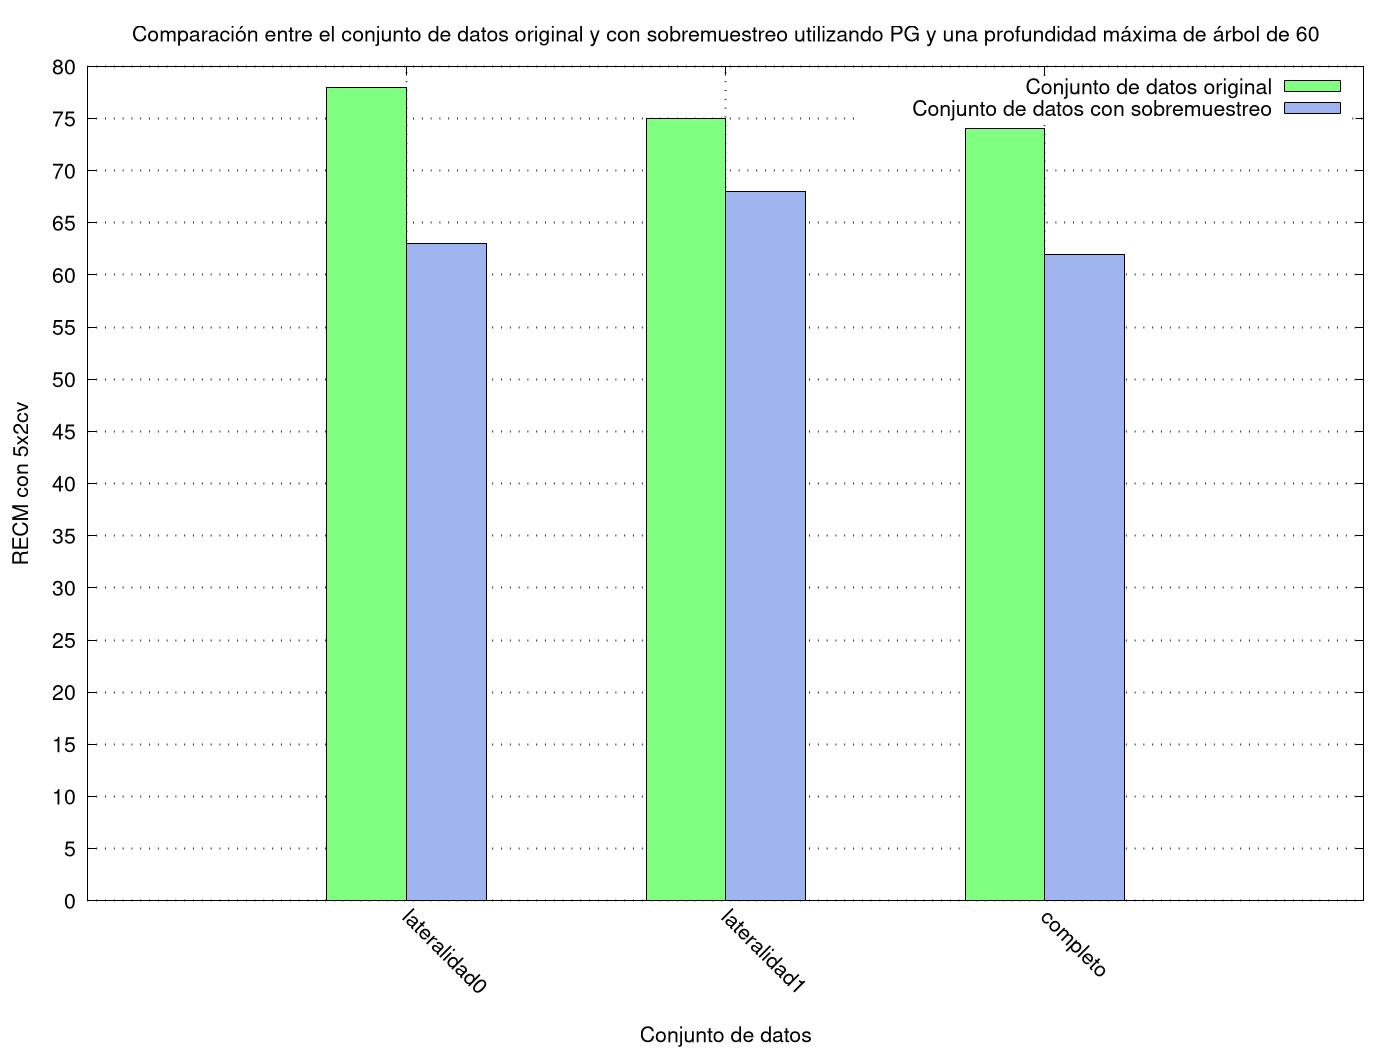
\includegraphics[width=0.7\textwidth]{analisis/comparacion_over_pg_60.png}
	  \caption{Comparación entre el conjunto de datos original y con sobremuestreo con PG y longitud máxima de 60 nodos.}\label{fig:cmp_pg_over_60}

\end{figure}

Estos cambios también son notables sobre GA-P:

\begin{figure}[H]
    \centering
	  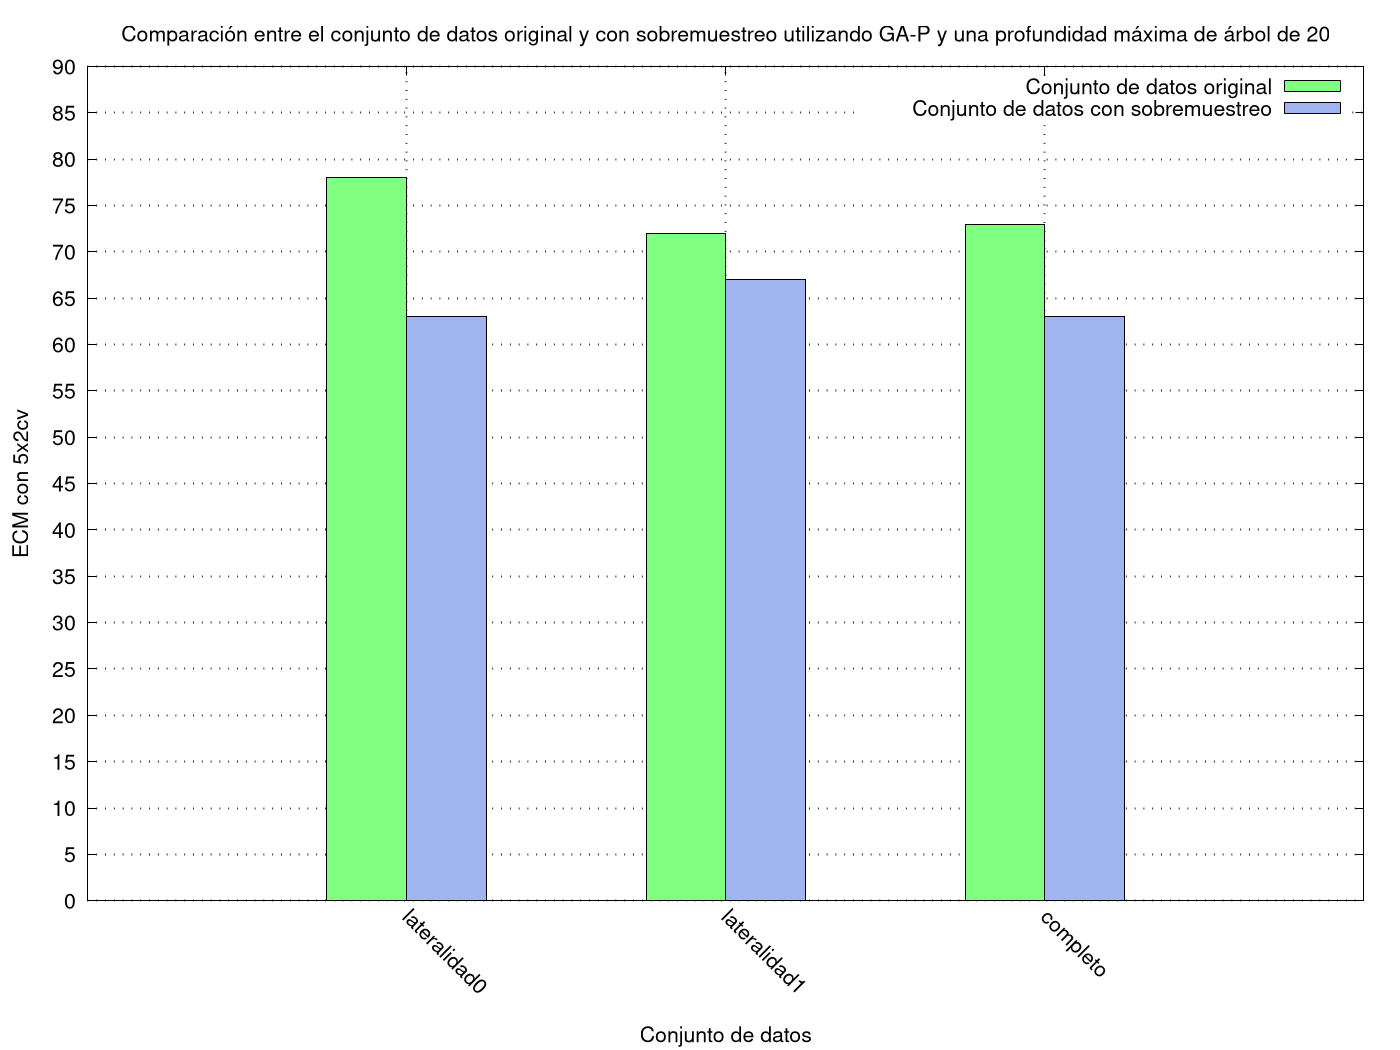
\includegraphics[width=0.7\textwidth]{analisis/comparacion_over_gap_20.png}
	  \caption{Comparación entre el conjunto de datos original y con sobremuestreo con GA-P y longitud máxima de 20 nodos.}\label{fig:cmp_gap_over_20}

\end{figure}

\begin{figure}[H]
    \centering
	  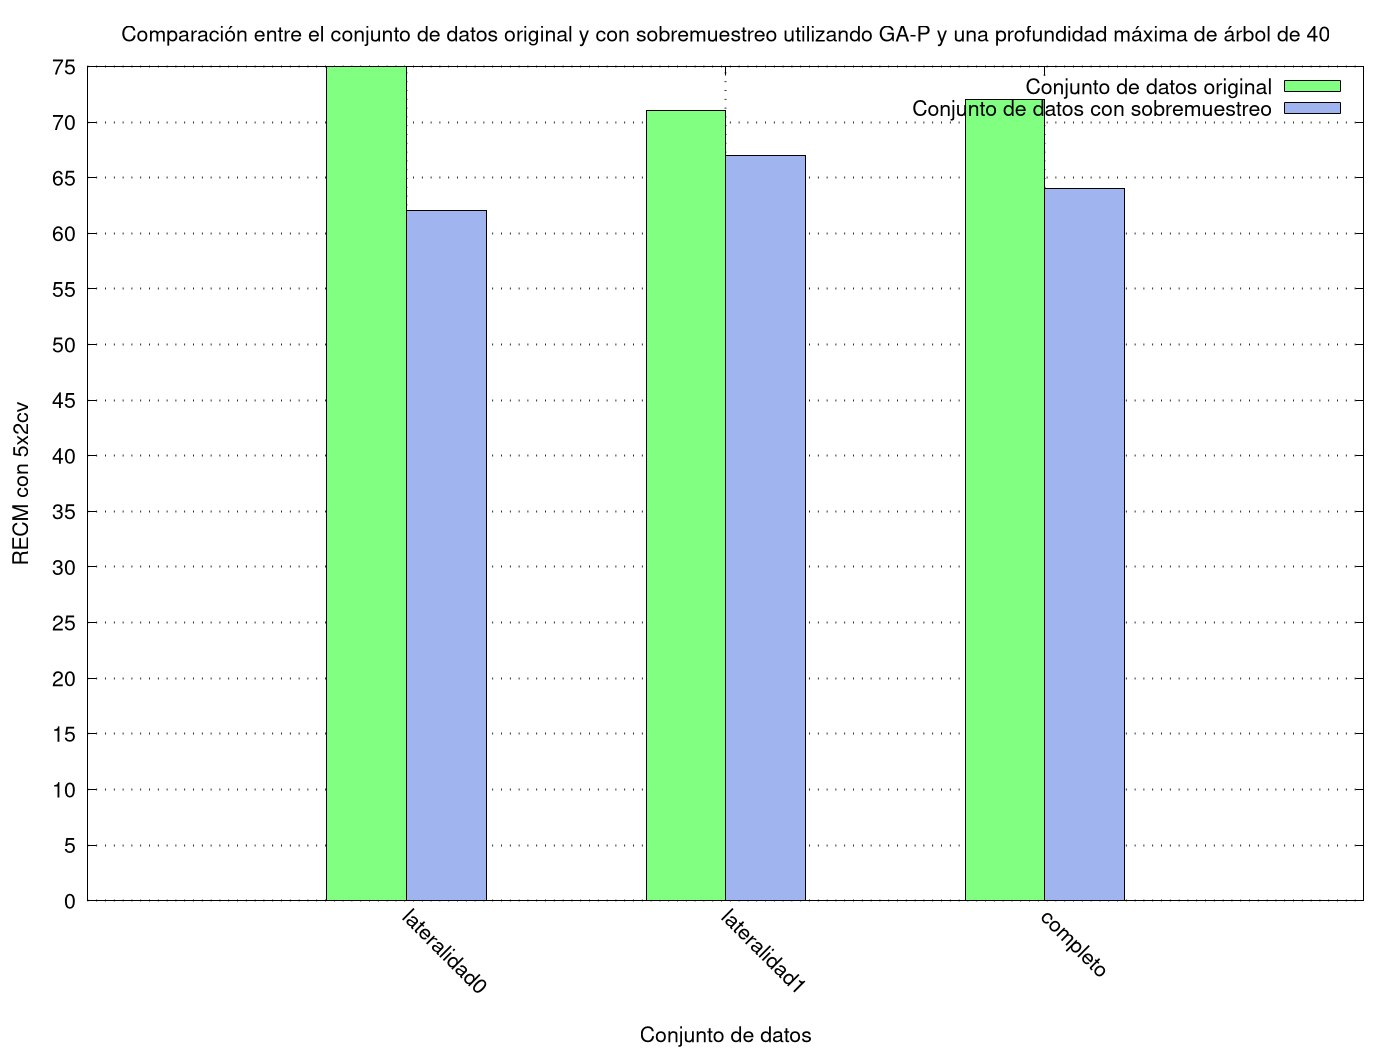
\includegraphics[width=0.7\textwidth]{analisis/comparacion_over_gap_40.png}
	  \caption{Comparación entre el conjunto de datos original y con sobremuestreo con GA-P y longitud máxima de 40 nodos.}\label{fig:cmp_gap_over_40}

\end{figure}

\begin{figure}[H]
    \centering
	  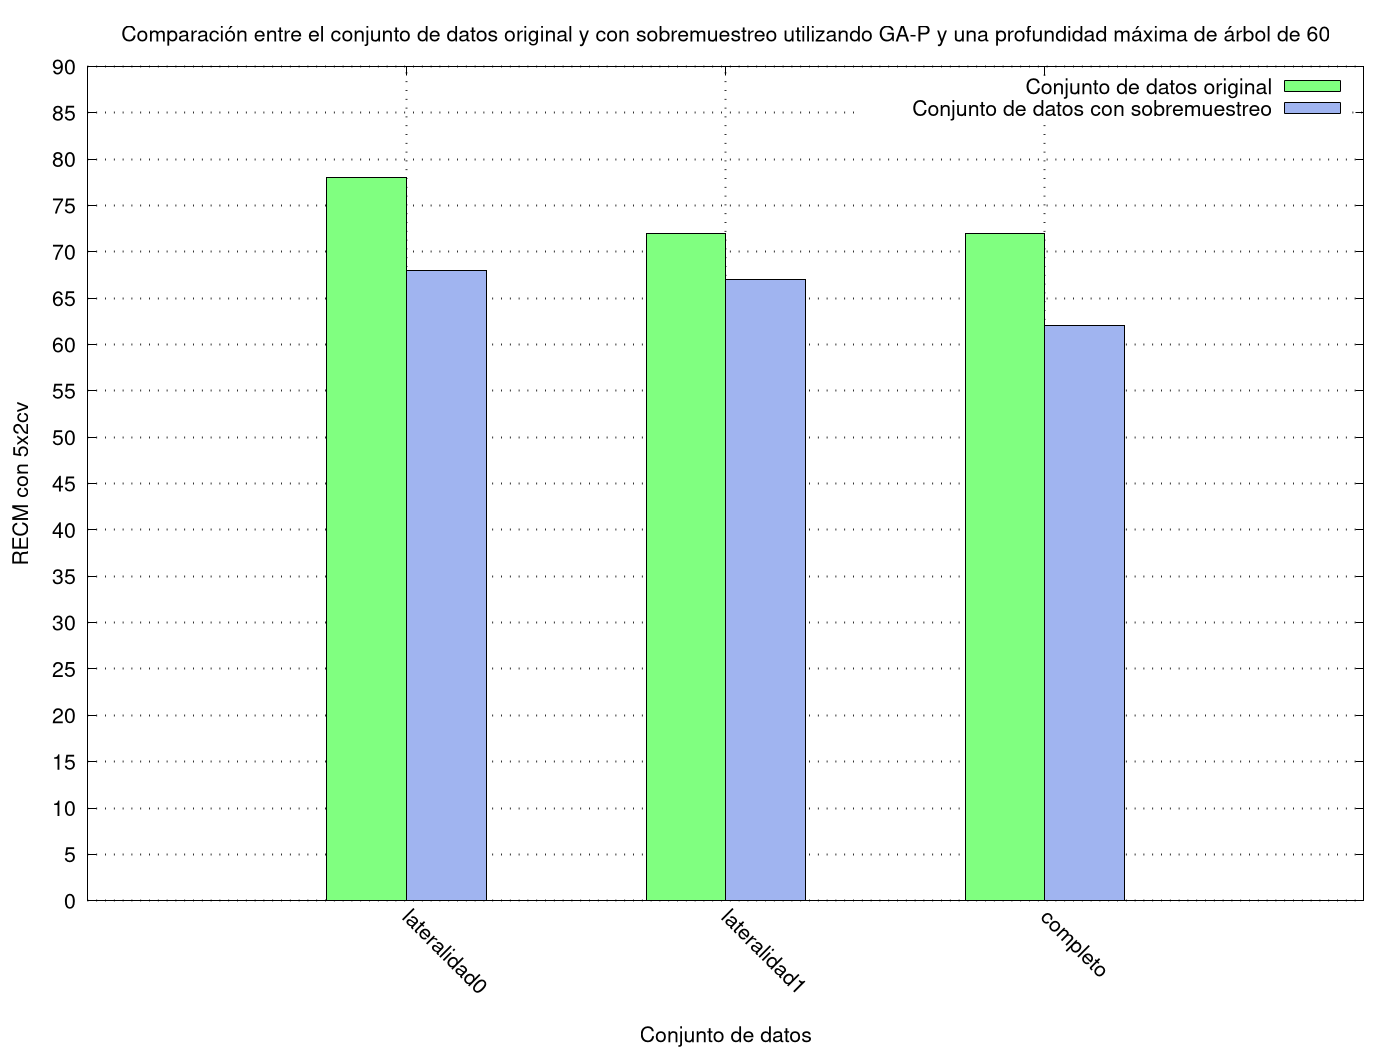
\includegraphics[width=0.7\textwidth]{analisis/comparacion_over_gap_60.png}
	  \caption{Comparación entre el conjunto de datos original y con sobremuestreo con GA-P y longitud máxima de 60 nodos.}\label{fig:cmp_gap_over_60}

\end{figure}

Como suponíamos al introducir el problema y el conjunto de datos a utilizar en la sección \ref{introduccion}, el conjunto de datos original no cuenta con suficientes datos para los valores de edades más tempranas, y el realizar el sobremuestreo explicado en la sección \ref{sobremuestreo} ha conseguido mejorar notablemente los resultados.

Estos resultados son una muestra de la importancia de trabajar con un buen conjunto de datos, así como de la importancia de buscar nuevas técnicas que nos permitan obtener datos sintéticos. Como se ha visto en el estado del arte y la explicación del sobremuestreo, SMOTE y sus variantes realizan una función clave en este tipo de problemas, donde obtener datos es una tarea compleja.

\subsection{Comparación con el estado del arte}

De cara a comparar con el estado del arte utilizaremos los resultados obtenidos por Gámez-Granados et al \cite{NSLVOrdAge} ya que se trata de un trabajo actual, donde se consiguen unos muy buenos resultados siendo los mejores del estado del arte actual, además de utilizar el mismo conjunto de datos utilizado en este trabajo pero con un enfoque de clasificación, y no de regresión, por lo que nos permitirá saber si modificar el enfoque original de Todd por el enfoque de Gilbert y McKern pero utilizando las características de Todd ha funcionado.

En este trabajo se obtienen los siguientes resultados:


\begin{table}[H]
\centering
% \resizebox{\textwidth}{!}{%
\begin{tabular}{|c|c|c|}
\hline
\multicolumn{3}{|c|}{\textbf{Mejores resultados del estado del arte}}        \\ \hline
\textbf{}                                     & \textbf{RECM} & \textbf{MAE} \\ \hline
\textbf{NSLVORD: Lateralidad izquierda}       & 12,486        & 9,412        \\ \hline
\textbf{NSLVORD: Lateralidad derecha}         & 12,558        & 9,596        \\ \hline
\textbf{Random Forest: Lateralidad izquierda} & 12,277        & 9,408        \\ \hline
\textbf{Random Forest: Lateralidad derecha}   & 11,372        & 8,298        \\ \hline
\end{tabular}%
% }
\caption{Resultados obtenidos de \cite{NSLVOrdAge}.}\label{table:resultados_estado_arte}
\end{table}

Como podemos ver en esta tabla \ref{table:resultados_estado_arte}, la propuesta hecha en \cite{NSLVOrdAge} iguala los resultados de técnicas más complejas como Random Forest, obteniendo unos resultados mucho más interpretables y útiles de cara a los forenses, llegando a mejorarlos al aplicar sobremuestreo, aunque en la publicación solo utilizan medidas de error para problemas de clasificación en el caso de los conjuntos de datos con sobremuestreo, de ahí que no aparezcan en la tabla.

En su trabajo también se habla de como su propuesta es capaz de obtener resultados mucho más interpretables, en los que se obtienen únicamente 34 reglas en comparación con las 1091 de Random Forest, por lo que podemos concluir que la aplicación de regresión simbólica hace más favorable esta situación, al tratarse de una única fórmula para cualquier dato disponible.

Tras revisar estos resultados, vamos a añadir los obtenidos en nuestros experimentos:


\begin{table}[H]
\centering
% \resizebox{\textwidth}{!}{%
\begin{tabular}{|c|c|c|}
\hline
\multicolumn{3}{|c|}{\textbf{Mejores resultados del estado del arte}}        \\ \hline
\textbf{}                                     & \textbf{RECM} & \textbf{MAE} \\ \hline
\textbf{NSLVORD: L. izquierda}                & 12,486        & 9,412        \\ \hline
\textbf{NSLVORD: L. derecha}                  & 12,558        & 9,596        \\ \hline
\textbf{Random Forest: L. izquierda}          & 12,277        & 9,408        \\ \hline
\textbf{Random Forest: L. derecha}            & 11,372        & 8,298        \\ \hline
\textbf{PG: L. izquierda}                     & 8,5315        & 7,076        \\ \hline
\textbf{PG: L. derecha}                       & 8,2147        & 6,738        \\ \hline
\textbf{GA-P: L. izquierda}                   & 8,5659        & 7,111        \\ \hline
\textbf{GA-P: L. derecha}                     & 8,2059        & 6,703        \\ \hline
\textbf{PG: L. izquierda (sobremuestreo)}     & 7,8646        & 6,394        \\ \hline
\textbf{PG: L. derecha (sobremuestreo)}       & 7,9840        & 6,559        \\ \hline
\textbf{GA-P: L. izquierda (sobremuestreo)}   & 7,8949        & 6,445        \\ \hline
\textbf{GA-P: L. derecha (sobremuestreo)}     & 8,1103        & 6,708        \\ \hline
\end{tabular}%
% }
\caption{Resultados obtenidos de \cite{NSLVOrdAge} en comparación con los de este trabajo.}\label{table:cmp_estado_arte}
\end{table}

De cara a la selección se ha buscado que la fórmula sea simple, y que tenga un buen resultado, no estrictamente la mejor, al buscar que esta sea interpretable fácilmente. Profundizaremos sobre esto en la siguiente sección.

Como vemos en \ref{table:cmp_estado_arte}, nuestro trabajo ha conseguido mejorar los resultados obtenidos hasta el momento para el problema de la estimación de la edad a través de los huesos del pubis, con un modelo fácil de interpretar y que sea simple, además de aplicar técnicas de sobremuestreo para seguir mejorando dichos resultados, haciendo que este enfoque sea de gran competencia y pueda añadir un gran valor a la hora de resolver este problema.

Con esto también podemos concluir que el enfocar el problema como un problema de regresión en lugar de clasificación, utilizar las características propuestas por Todd de cara a obtener un mayor grado de libertad y utilizar algoritmos capaces de aprender dicho grado de libertad, ha permitido sacar el máximo provecho al conjunto de datos disponible, permitiendo una gran flexibilidad al escoger las características utilizadas y eliminando el sesgo que se podría introducir con cualquier otro método al no tener que escoger la forma del resultado.


\subsection{Análisis de las expresiones obtenidas y mejores expresiones}


Tras comparar los distintos algoritmos, los conjuntos de datos utilizados y revisar el estado del arte en comparación con nuestra propuesta, en esta sección se analizará de forma general los detalles más importantes de los resultados obtenidos, así como mostrar las mejores expresiones obtenidas por cada algoritmo en cada conjunto de datos de cara a analizarlas en profundidad.

\subsubsection{Mejores expresiones obtenidas}

En esta sección seleccionaremos cuatro fórmulas, una por cada algoritmo utilizado con y sin sobremuestreo sobre el conjunto de datos completo, con el objetivo de escoger los mejores resultados y más sencillos para su interpretación. Debido a que las fórmulas que utilizan como máximo veinte nodos de longitud para los árboles son más simples y se han obtenido resultados similares con distintas longitudes máximas, me limitaré a estas ya que queremos que el resultado sea interpretable.

\begin{equation} \label{eq:PG_completo}
10,856454 x_{4} + 5,428227 x_{8} + 8,374907 - \frac{3,803607512943}{x_{1}^{3}}
\end{equation}


\begin{equation} \label{eq:GAP_completo}
2,330831 x_{1} + 8,270077 x_{8} + \left(x_{0} - x_{8}\right) \left(x_{8} - 2,330831\right) + 16,945320843987
\end{equation}


\begin{equation} \label{eq:PG_completo_over}
3.2443 x_{1} - 3.2443 x_{3} + x_{4}^{2} + 2.5906246154344 x_{4} x_{8} + 22.5431061461
\end{equation}


\begin{equation} \label{eq:GAP_completo_over}
3.030219 x_{1} + 5.632281 x_{4} + 5.204124 x_{8} + 12.212446187961
\end{equation}

\ref{eq:PG_completo} se trata de la mejor fórmula obtenida con Programación Genética sobre el conjunto de datos completo sin sobremuestreo, \ref{eq:GAP_completo} la mejor fórmula con GA-P sobre el conjunto de datos sin sobremuestreo, \ref{eq:PG_completo_over} la mejor fórmula de Programación Genética con sobremuestreo, y \ref{eq:GAP_completo_over} la mejor fórmula de GA-P con sobremuestreo.

Los resultados individuales de estas fórmulas son los siguientes:


\begin{table}[]
\centering
% \resizebox{\textwidth}{!}{%
\begin{tabular}{|c|c|c|}
\hline
\multicolumn{3}{|c|}{\textbf{Resultados de las expresiones escogidas}}   \\ \hline
\textbf{}                       & \textbf{RECM}    & \textbf{MAE}        \\ \hline
\textbf{PG}                     & 8,39821          & 6,92052             \\ \hline
\textbf{GA-P}                   & 8,4945           & 6,96785             \\ \hline
\textbf{PG con sobremuestreo}   & 7,8669           & 6,41288             \\ \hline
\textbf{GA-P con sobremuestreo} & 7,87184          & 6,42334             \\ \hline
\end{tabular}%
% }
\caption{Resultados de las expresiones \ref{eq:PG_completo}, \ref{eq:GAP_completo}, \ref{eq:PG_completo_over} y \ref{eq:GAP_completo_over}.}\label{table:resultados_escogidas}
\end{table}

Estos resultados se encuentra un poco por debajo de la media global, aunque no se tratan de las mejores con el objetivo de que sean fórmulas simples.

Todas las fórmulas obtenidas tienen algo en común, la presencia de la última característica ($x_8$), el borde ventral, de la quinta característica ($x_4$), el borde inferior (a excepción de \ref{eq:GAP_completo}) y de la segunda característica $x_1$, la superficie porosa irregular (a excepción de \ref{eq:PG_completo}). En un principio con esto podríamos deducir que forman una parte importante en el proceso de estimación de la edad, aunque lo veremos más a fondo en la siguiente sección.



\subsubsection{Uso de características}

Como comentamos en la sección anterior, hay algunas características que son más usadas que otras. En esta sección estudiaremos que características son las más utilizadas y revisaremos el estado del arte para comprobar si las variables más utilizadas coinciden con lo esperado.

De cara a realizar este estudio, a partir de todas las fórmulas obtenidas en las distintas ejecuciones se han contado el número de apariciones de cada característica:

\begin{table}[H]
\centering
\resizebox{\textwidth}{!}{%
\begin{tabular}{|c|c|c|c|c|c|c|c|c|c|c|}
\hline
\multicolumn{11}{|c|}{\textbf{Uso de variables}}                                                                                                                                                                                              \\ \hline
                              & $\boldsymbol{x_0}$   & $\boldsymbol{x_1}$   & $\boldsymbol{x_2}$  & $\boldsymbol{x_3}$  & $\boldsymbol{x_4}$   & $\boldsymbol{x_5}$  & $\boldsymbol{x_6}$  & $\boldsymbol{x_7}$  & $\boldsymbol{x_8}$   & \textbf{\begin{tabular}[c]{@{}c@{}}Número total \\ de características\end{tabular}} \\ \hline
\textbf{PG}                   & 46               & 94               & 14              & 8               & 64               & 12              & 42              & 57              & 105              & \textbf{442}                            \\ \hline
\textbf{GA-P}                 & 48               & 93               & 20              & 10              & 68               & 14              & 60              & 42              & 85               & \textbf{440}                            \\ \hline
\textbf{PG sobremuestreo}     & 54               & 94               & 13              & 17              & 67               & 18              & 29              & 22              & 97               & \textbf{411}                            \\ \hline
\textbf{GA-P sobremuestreo}   & 44               & 80               & 25              & 21              & 67               & 35              & 27              & 29              & 86               & \textbf{414}                            \\ \hline
\textbf{Total}                & \textbf{192}     & \textbf{361}     & \textbf{72}     & \textbf{56}     & \textbf{266}     & \textbf{79}     & \textbf{158}    & \textbf{150}    & \textbf{373}     & \textbf{1707}                           \\ \hline
\textbf{\% respecto al total} & \textbf{11,25\%} & \textbf{21,15\%} & \textbf{4,22\%} & \textbf{3,28\%} & \textbf{15,58\%} & \textbf{4,63\%} & \textbf{9,26\%} & \textbf{8,79\%} & \textbf{21,85\%} & \textbf{}                               \\ \hline
\end{tabular}%
}
\caption{Uso de las características en todas las fórmulas obtenidas dividido por algoritmo y sobremuestreo.}\label{table:uso_caracteristicas}
\end{table}

En total se han realizado ejecuciones en dos algoritmos (Programación Genética y GA-P), con tres longitudes máximas cada uno ($20$, $40$, y $60$ nodos como longitud máxima del árbol), con seis conjuntos de datos distintos (lateralidad izquierda, derecha, conjunto completo y estos tres con oversampling) y con cinco semillas distintas, lo que supone que hemos obtenido $180$ fórmulas distintas, cada una de ellas independientes, como resultado.

Suponiendo que las fórmulas utilizan su longitud de árbol, son un total de $7.200$ nodos ($1.200$ nodos de las expresiones de longitud máxima $20$ nodos, $2.400$ de expresiones con longitud máxima $40$ y $3.600$ de expresiones con longitud máxima $60$), de los cuales, como podemos ver en la tabla \ref{table:uso_caracteristicas}, sabemos que en total de $1.707$ son características, un $47,41\%$ del número máximo de posibles nodos suponiendo que todas las expresiones llegan a este máximo.

Con respecto al uso concreto de cada variable, la más utilizada es la características $x_8$, el borde ventral, seguida de la segunda variable, $x_1$, la superficie porosa irregular, ambas con más de un $20\%$ de apariciones en el total de $180$ fórmulas, con una aparición del $21.85$ y del $21,15$ respectivamente. Además de estas dos variables, otra que destaca es el borde inferior, $x_4$, apareciendo un $15,58\%$ de las ocasiones que aparece un nodo de variable.

Unicamente estas tres variables del total de nueve suponen casi un $60\%$ de todas las características utilizadas en las $180$ expresiones totales obtenidas, por lo que podemos afirmar que se tratan de variables de gran interés a la hora de estimar la edad de los individuos.

Por otro lado, entre las menos utilizadas encontramos el nódulo óseo, $x_3$, el borde superior, $x_2$ y el borde dorsal, $x_6$, utilizados apenas un $3,28\%$, $4,22\%$ y $4,63\%$ respectivamente. En este caso, un tercio del total de características apenas llegan a aparecer un poco más del $12\%$.

Además de dicha frecuencia de uso tan baja, en otros trabajos que han tratado este problema como \cite{NSLVOrd} han llegado a la conclusión de que ciertas variables no intervienen en el proceso de estimación de la edad, como por ejemplo el borde dorsal o el borde superior, coincidiendo con nuestros resultados. Por este motivo, podemos llegar a la conclusión de que se podrían reducir el número de características a utilizar de cara a reducir el tamaño del problema ya que algunas de las variables propuestas por Todd no influyen en el problema.



\subsubsection{Aportaciones de técnicas de inteligencia artificial explicables al problema}


\newpage
